

\chapter{Introduction} % Main chapter title

\label{Chapter 1} 
\lhead{Chapter 1. \emph{Introduction}} 


There are following eight forms of dance recognized by the Sangeet Natak Akademi \citep{wiki:004}.

\begin{enumerate}
    \item Bharatanatyam
    \item Kathakali
    \item Odissi
    \item Kathak
    \item Kuchipudi
    \item Mohiniyattam
    \item Manipuri
    \item Sattriya
\end{enumerate}

These all dance types represent South Indian religious texts and religious beliefs, especially of Shaivism, Vaishnavism and Shaktism. \citep{williams2004shadow}

Bharatanatyam is a important form of IDC (Indian classical dance) that began in the state of Tamil Nadu hundreds of years ago. \citep{williams2004shadow}. Its origin can be traced back to the Natya Sastra. It is a Sanskrit text written by sage Bharata Muni on the performing arts. Bharatnatyam  was originated of two words, ‘Bharata’ and ’Natyam’, where 'Bharata' is a mnemonic containing ‘bha’, ‘ra’ and ‘ta’ which respectively.
Here ‘bhava’ is emotion and feelings; ‘raga’ is a melody, and ‘tala’ beats.
In Hindus temples, Bharatanatyam was exclusive up to the $19^th$ century. In modern days, Bharatanatyam spread out to different parts of India and available on the internet easily.
 
 Bharatanatyam dance movements are portrayed by bent legs, while feet keep beat. In a set of mudras, symbolic hand gestures are used to express a story.
 
 Bharatanatyam have basic choreographic units of a dance sequence. An Adavu is accompanied by percussion and vocal music and follows a specific rhythmic pattern \citep{mallick2018characterization}.

 \begin{figure}
    \centering
    \subfigure[]{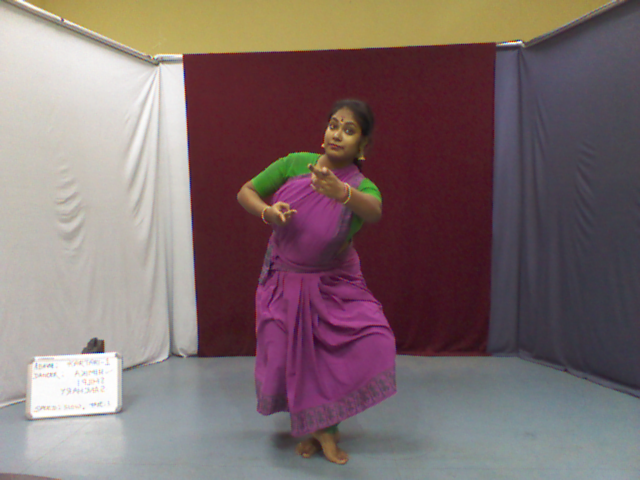
\includegraphics[width=0.32\textwidth]{Pictures/color_USB-VID_045E&PID_02BF-0000000000000000_239.png}} 
    \subfigure[]{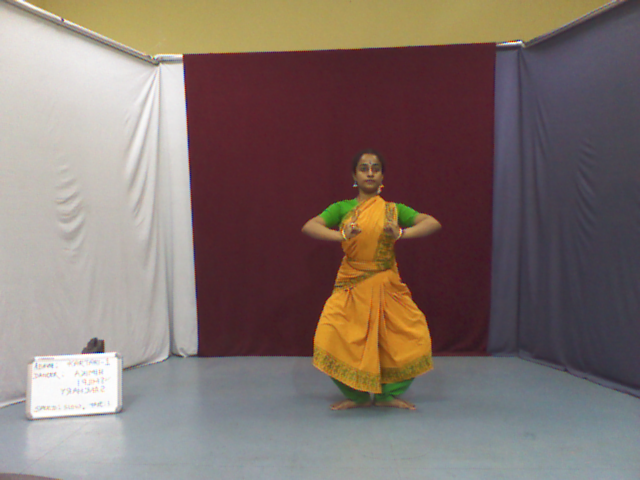
\includegraphics[width=0.32\textwidth]{Pictures/color_USB-VID_045E&PID_02BF-0000000000000000_74.png}} 
    \subfigure[]{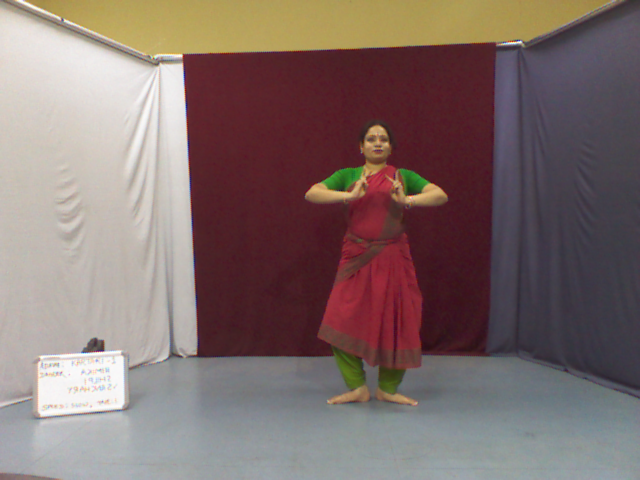
\includegraphics[width=0.32\textwidth]{Pictures/color_USB-VID_045E&PID_02BF-0000000000000000_14.png}}
    \caption{(a) Dancer 1 (b) Dancer 2 (c) Dancer 3}
    \caption{Bharatanatyam, Katti kartari Adavu, Variation 1}
    \label{fig:Ch01001}
\end{figure}

There are following classification of Adavus in Bharatnatyam. There are multiple variations under Adavus in Bharatnatyam.
\begin{enumerate}
    \item Tattu Adavu
    \item Nattu Adavu
    \item Pakka Adavu
    \item Kudditu Mettu Adavu
    \item Kudditu Nattal Adavu
    \item Kudditu Tattal Adavu
    \item Paikal Adavu
    \item Tei Tei Dhatta
    \item Katti Kartari as shown in Figure \ref{fig:Ch01001}
    \item Utsanga Adavu
    \item Mandi Adavu
    \item Sarrikkal Adavu
    \item Tirmana Adavu
    \item Sarika Adavu
    \item Joining Adavu
\end{enumerate}

\section{Bharatnatyam \& Computer Vision}
Bharatnatyam contains a large number of motion frames and Key Postures.

In Computer Vision, Human motion, representation and  its characteristic is an important topic. They are represented and displayed in various forms through centuries.
Human identification using motion analysis is mainly focused on observing human gait.
The motion of a person's legs and motion of a person's arms are considered as human gait.
There is motion information available in dance frames of Adavus. So, 
a high-level feature representation of the dance frame has used using Histogram of optical flow (HOOF).

There are following dancers as shown in Figure \ref{fig:Ch01001}, for Katti Kartari Adavu in Variation 1.


 


Following important terminology are associated with \textbf{Bharatanatyam Dance}:
\begin{itemize}
    \item \textbf{Adavu:} The basic unit of Bharatanatyam.
    \item \textbf{Key Postures(KP):} Momentarily stationary well-defined postures occur within the Adavu
    \item \textbf{Key Frames(KF):} Frames associated with a Key Posture
    \item \textbf{Motion Frames(MF):} Frames associated with motion
\end{itemize}

\section{Introduction to Keyframe and motion frame in Bharatanatyam}


\begin{figure}[H]
  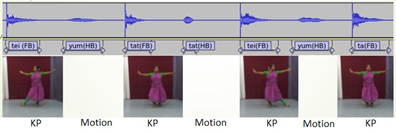
\includegraphics[scale= 1]{./Pictures/motion_fig.png}
  \caption{Occurrence of Motion and KPs}
  \label{fig:Ch1F004}
\end{figure}

There are various steps involved in Bharatanatyam dance. 
In Bharatanatyam, the dancer takes momentarily stationary well-defined posture, which occurs within each Adavus followed by sophisticated or complex motions frames. These are called Key Posture (KP).
Then, there are some frames associated with a Key Posture. They are called Key Frames.
During the dance, there is a transition from one Key Posture to the next Key Posture. They are called Motion (M). Motions (M) and Key Postures (KP) occur alternately and may repeat in a Bharatanatyam dance performance. Suppose there is Bharatanatyam dance Performance P, which consists of the interleaving sequence of Keyframes and motion frames like K1 M1 K2 M2 K3 M3 ... K(n-1) M(n-1) Kn. Where K is Keyframe, M is a motion frame,1,2,3...,n is $1^st$, $2^nd$, $3^rd$, ..., $n^th$ Keyframe or motion frame and n is the total frame. A motion comprised of several set of frames those are not momentarily stationary.




















